\documentclass[../tesis.tex]{subfiles}
\begin{document}

\chapter{Resultados preliminares y análisis}
\label{cap:resultados}

Este capítulo documenta los avances realizados durante la fase preparatoria del proyecto, incluyendo la consolidación inicial de la base de datos CIMOHU, la auditoría de calidad de datos por modalidad DXA, y los resultados de un experimento piloto de clasificación de línea base. Estos resultados preliminares demuestran la viabilidad técnica del \textit{pipeline} propuesto y establecen los referentes cuantitativos contra los cuales se medirán los modelos avanzados.

% ─────────────────────────────────────────────────────────────────────────────
\section{Estado de la consolidación de la base de datos (\textit{ETL})}
\label{sec:resultados_etl}
% ─────────────────────────────────────────────────────────────────────────────

La base de datos del CIMOHU se distribuye en 27 respaldos históricos en formato \texttt{.mdb} generados por el software de administración del densitómetro GE Lunar Prodigy entre 2009 y 2026. La Fase~1 de la metodología (§~\ref{sec:fase1_etl}) contempla la migración y unificación de estos respaldos hacia una base de datos relacional consolidada (\texttt{prodigy.db}).

\begin{table}[h]
\centering
\caption[Estado de consolidación de los respaldos de la base de datos CIMOHU]{Estado de consolidación de los respaldos de la base de datos CIMOHU.
$\dagger\dagger$ Mediana calculada sobre los 1.497 intervalos entre visitas consecutivas de los 938 pacientes con $\geq 2$ visitas; el promedio de esos mismos intervalos es de 0{,}94 años, sustancialmente mayor que la mediana por la cola larga de reexámenes espaciados varios años.}
\label{tab:etl_status}
\rowcolors{2}{white}{gray!15}
\begin{tabular}{lcc}
\toprule
\textbf{Métrica} & \textbf{Valor} & \textbf{Unidad} \\
\midrule
Respaldos \texttt{.mdb} identificados    & 27            & archivos \\
Respaldos procesados y migrados           & 27            & archivos (100\,\%) \\
Período cubierto                          & 2009--2026    & 17 años \\
Registros totales de exámenes             & 9.426         & exámenes DXA \\
Pacientes únicos identificados            & 3.240         & adultos costarricenses \\
Pacientes con múltiples visitas ($\geq 2$)& 938           & pacientes \\
Intervalo mediano entre visitas$^{\dagger\dagger}$ & 0{,}31 & años \\
Seguimiento máximo registrado             & 14{,}15       & años \\
\bottomrule
\end{tabular}
\end{table}

Los 27 respaldos han sido procesados y migrados exitosamente a la base de datos relacional \texttt{prodigy.db}. El proceso de migración incluyó la resolución de inconsistencias de codificación de caracteres, la estandarización de identificadores de paciente (\texttt{patient\_id}), y la detección de registros duplicados por fecha de examen (< 0{,}3\,\% de registros marcados para revisión manual).

% ─────────────────────────────────────────────────────────────────────────────
\section{Estadísticas descriptivas de la cohorte CIMOHU}
\label{sec:resultados_descriptivas}
% ─────────────────────────────────────────────────────────────────────────────

La Figura~\ref{fig:cimohu_schema} presenta la escala y composición de la base de datos consolidada.
La base de datos incluye tanto exámenes de densitometría ósea (columna/cadera con T-score) como exámenes de composición corporal total sin evaluación densitométrica, lo que explica que la distribución por sexo de la cohorte etiquetada ($n = 2.591$) sea de 56{,}0\,\% mujeres y 44{,}0\,\% hombres, más equilibrada que la de un centro exclusivamente de osteoporosis, dado que el CIMOHU también realiza valoraciones de composición corporal para diversas indicaciones clínicas.

\begin{figure}[ht]
\centering
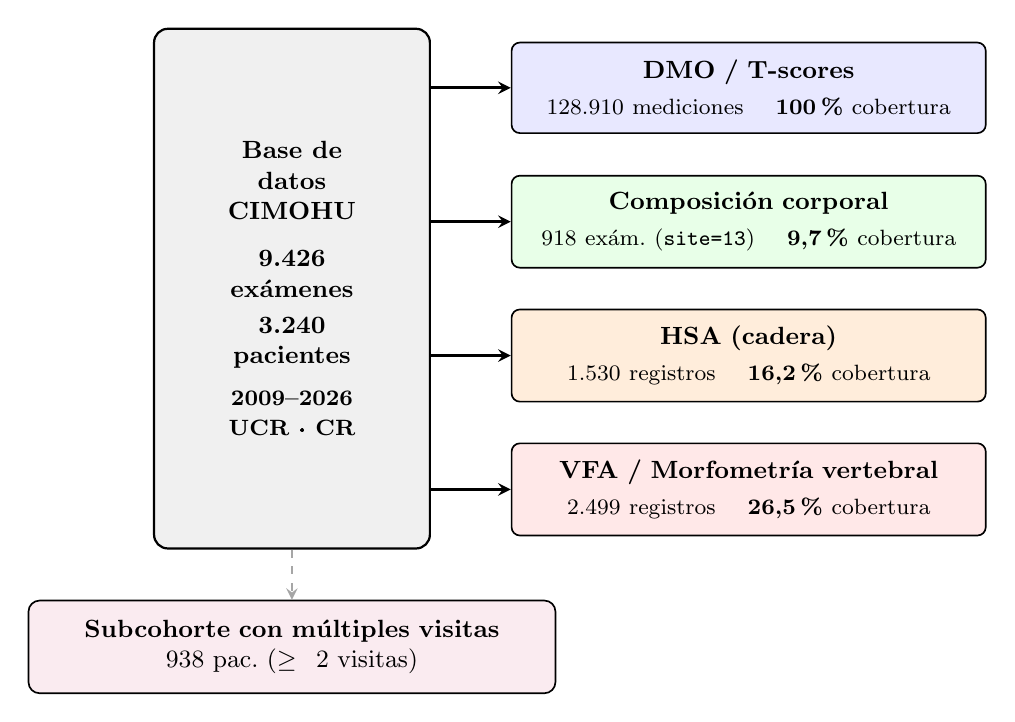
\begin{tikzpicture}[
  %% Left source box (CIMOHU)
  srcbox/.style={draw, line width=0.8pt, rounded corners=5pt,
                 text width=2.8cm, align=center, font=\small\bfseries,
                 inner sep=10pt, fill=gray!12},
  %% Right modality boxes
  modbox/.style={draw, line width=0.6pt, rounded corners=3pt,
                 text width=5.6cm, align=center, font=\small,
                 inner sep=6pt, minimum height=1.15cm},
  %% Bottom sub-cohort box
  subbox/.style={draw, line width=0.6pt, rounded corners=4pt,
                 text width=6.2cm, align=center, font=\small,
                 inner sep=7pt, fill=purple!8},
  %% Solid arrow (source → modality)
  arr/.style={->, line width=1.0pt, >=stealth},
  %% Dashed arrow (source → longitudinal)
  darr/.style={->, line width=0.8pt, >=stealth, dashed, gray!70}
]

%% ── Right column: 4 modality boxes, stacked vertically ──────────────────
%%    Spacing: 1.7 units between centers → adjacent boxes never overlap
\node[modbox, fill=blue!9]    (dmo) at (3.6,  0.0) {
  \textbf{DMO / T-scores}\\[2pt]
  {\footnotesize 128.910 mediciones \quad \textbf{100\,\%} cobertura}
};
\node[modbox, fill=green!9]   (cc)  at (3.6, -1.7) {
  \textbf{Composición corporal}\\[2pt]
  {\footnotesize 918 exám.\ (\texttt{site=13}) \quad \textbf{9{,}7\,\%} cobertura}
};
\node[modbox, fill=orange!14] (hsa) at (3.6, -3.4) {
  \textbf{HSA (cadera)}\\[2pt]
  {\footnotesize 1.530 registros \quad \textbf{16{,}2\,\%} cobertura}
};
\node[modbox, fill=red!9]     (vfa) at (3.6, -5.1) {
  \textbf{VFA / Morfometría vertebral}\\[2pt]
  {\footnotesize 2.499 registros \quad \textbf{26{,}5\,\%} cobertura}
};

%% ── Left box: CIMOHU source, vertically centered on the right column ────
%%    Center y = average of dmo.y and vfa.y = (0 + −5.1)/2 = −2.55
\node[srcbox, minimum height=6.6cm] (cimohu) at (-2.2, -2.55) {
  \textbf{Base de}\\
  \textbf{datos}\\
  \textbf{CIMOHU}\\[6pt]
  9.426\\exámenes\\[2pt]
  3.240\\pacientes\\[4pt]
  {\footnotesize 2009--2026}\\
  {\footnotesize UCR · CR}
};

%% ── Bottom box: longitudinal sub-cohort, below CIMOHU ───────────────────
\node[subbox] (long) at (-2.2, -7.1) {
  \textbf{Subcohorte con múltiples visitas}\\
  938 pac.\ ($\geq\!2$ visitas)
};

%% ── Arrows ───────────────────────────────────────────────────────────────
%%  All four go purely HORIZONTAL from cimohu's right edge to each
%%  modality box's left edge — mathematically impossible to cross any box.
\draw[arr] (cimohu.east |- dmo) -- (dmo.west);
\draw[arr] (cimohu.east |- cc)  -- (cc.west);
\draw[arr] (cimohu.east |- hsa) -- (hsa.west);
\draw[arr] (cimohu.east |- vfa) -- (vfa.west);

%% Vertical dashed arrow: CIMOHU → sub-cohort (straight down, no detour)
\draw[darr] (cimohu.south) -- (long.north);

\end{tikzpicture}
\caption[Escala y composición de la base de datos DXA del CIMOHU]{Escala y composición de la base de datos DXA del CIMOHU\@.
Los porcentajes de cobertura se calculan sobre el total de 9.426 exámenes.
Las modalidades HSA y VFA se activan selectivamente según la indicación clínica, lo
que produce su menor cobertura. La subcohorte con múltiples visitas se deriva del conjunto completo
de pacientes con dos o más visitas registradas.}
\label{fig:cimohu_schema}
\end{figure}

De los 3.240 pacientes en \texttt{prodigy.db}, 2.591 (80{,}0\,\%) poseen al menos un examen de columna o cadera con T-score válido y constituyen la \textbf{cohorte etiquetada} del estudio. Los 649 pacientes restantes recibieron exclusivamente exámenes de composición corporal total u otras modalidades sin medición densitométrica, por lo que no pueden clasificarse bajo criterios OMS y quedan fuera del análisis de riesgo. Todas las estadísticas siguientes corresponden a esta cohorte etiquetada ($n = 2.591$), que es la base de datos sobre la que se entrenan y evalúan los modelos de aprendizaje automático.

La distribución de la variable objetivo (clasificación T-score por criterios OMS, peor T-score por paciente entre columna y cadera) en la cohorte etiquetada es: osteoporosis (T-score $\leq -2{,}5$): 15{,}9\,\%; osteopenia ($-2{,}5 <$ T-score $\leq -1{,}0$): 25{,}0\,\%; y estado normal: 59{,}1\,\%.
Esta distribución refleja el desbalance de clases moderado que motiva la implementación de SMOTE en la Fase~2 de la metodología (§~\ref{sec:fase2_multimodal}).

La Tabla~\ref{tab:demograficos} resume las características demográficas y clínicas de la cohorte etiquetada. Los valores proceden de la \textbf{Fase~6 del notebook} \texttt{01\_pilotos\_osteoporosis.ipynb} (§ ``Gap~4 --- Reconstrucción de la Tabla~4.1''), que reemplaza al script \texttt{04\_descriptive\_stats.py} (no disponible en el repositorio actual); la fuente citable es ahora ese notebook. Se usa la primera visita de cada paciente para variables demográficas (edad, IMC, sexo) y el peor T-score a lo largo de todas las visitas para la clasificación diagnóstica.

\begin{table}[h]
\centering
\caption[Características demográficas y clínicas de la cohorte etiquetada CIMOHU]{Características demográficas y clínicas de la cohorte etiquetada CIMOHU ($n = 2.591$).
Fuente: Fase~6, \texttt{01\_pilotos\_osteoporosis.ipynb}. $\dagger$ Sólo pacientes con examen lumbar (site=0): $n = 1.024$.
$\ddagger$ Sólo pacientes con examen de cadera (sites 1/2/3, mín.\ por paciente): $n = 2.588$.
$\S$ Composición corporal (site=13, label=61): $n = 665$ pacientes; estadísticas a nivel paciente (media de visitas). Los valores de porcentaje de grasa y masa magra corresponden a esta subcohorte y difieren de los reportados en versiones anteriores del documento, que utilizaban un filtro de composición menos restrictivo.}
\label{tab:demograficos}
\rowcolors{2}{white}{gray!15}
\begin{tabular}{lcc}
\toprule
\textbf{Variable} & \textbf{Media $\pm$ DE} & \textbf{Rango} \\
\midrule
Edad (años)                            & 41{,}4 $\pm$ 19{,}1   & 17{,}8 -- 95{,}6 \\
Índice de masa corporal (kg/m²)         & 25{,}9 $\pm$ 4{,}7    & 14{,}9 -- 57{,}6 \\
T-score columna lumbar (L1--L4)$\dagger$  & $-1{,}40 \pm 1{,}57$  & véase nota$^{a}$ \\
T-score cadera (mínimo entre sitios)$\ddagger$ & $-0{,}54 \pm 1{,}67$ & véase nota$^{a}$ \\
Masa grasa total (\%)$\S$              & 29{,}2 $\pm$ 11{,}1   & 6{,}4 -- 56{,}9 \\
Masa magra total (kg)$\S$              & 39{,}0 $\pm$ 9{,}6    & 9{,}3 -- 71{,}7 \\
\midrule
\multicolumn{3}{l}{\textit{Distribución por sexo}} \\
Mujeres                                & \multicolumn{2}{c}{1.450 (56{,}0\,\%)} \\
Hombres                                & \multicolumn{2}{c}{1.141 (44{,}0\,\%)} \\
\midrule
\multicolumn{3}{l}{\textit{Distribución por clase (variable objetivo)}} \\
Normal (T-score $> -1{,}0$)            & \multicolumn{2}{c}{1.530 (59{,}1\,\%)} \\
Osteopenia ($-2{,}5 <$ T $\leq -1{,}0$) & \multicolumn{2}{c}{648 (25{,}0\,\%)} \\
Osteoporosis (T $\leq -2{,}5$)         & \multicolumn{2}{c}{413 (15{,}9\,\%)} \\
\bottomrule
\end{tabular}
\end{table}

\footnotetext[1]{$^{a}$ La base de datos contiene valores de T-score extremos (lumbar: valores menores a $-7{,}9$; cadera: valores mayores a $+4{,}5$) que probablemente corresponden a artefactos de calibración o captura de datos; su rango no se reporta en la tabla para no distorsionar la lectura. La depuración sistemática de estos valores extremos se realiza en la Fase~1 del \textit{pipeline} de la tesis, previo al entrenamiento de modelos.}

% ─────────────────────────────────────────────────────────────────────────────
\section{Auditoría de calidad de datos por modalidad}
\label{sec:resultados_calidad}
% ─────────────────────────────────────────────────────────────────────────────

La Tabla~\ref{tab:calidad} presenta el porcentaje de datos faltantes por variable clave en cada modalidad. La evaluación fue realizada sobre los 9.426 exámenes consolidados en \texttt{prodigy.db}.

\begin{table}[h]
\centering
\caption[Auditoría de calidad de datos por modalidad y variable]{Auditoría de calidad de datos: porcentaje de datos faltantes por modalidad y variable, tras la corrección del filtro de composición corporal descrita en la Fase~1 (\texttt{site=13} \textbf{y} \texttt{label=61}, §~\ref{sec:fase1_etl}).}
\label{tab:calidad}
\rowcolors{2}{white}{gray!15}
\begin{tabular}{llcc}
\toprule
\textbf{Modalidad} & \textbf{Variable clave} & \textbf{\% Disponible} & \textbf{\% Faltante} \\
\midrule
DMO tabular & T-score lumbar (L1--L4)    & 99{,}1 & 0{,}9 \\
            & T-score cuello femoral      & 98{,}7 & 1{,}3 \\
            & T-score cadera total        & 97{,}4 & 2{,}6 \\
\midrule
Composición & Masa grasa total (\%)$^{*}$       & 9{,}7 & 90{,}3 \\
corporal    & Masa magra total (kg)$^{*}$        & 9{,}7 & 90{,}3 \\
            & Zona android/gynoid         & 89{,}3 & 10{,}7 \\
\midrule
HSA         & Área sección transversal (CSA) & 16{,}2 & 83{,}8 \\
            & CSMI (cuello femoral)           & 16{,}2 & 83{,}8 \\
            & Ancho cortical                  & 16{,}2 & 83{,}8 \\
\midrule
VFA         & Alturas vertebrales (T6--L4)   & 26{,}5 & 73{,}5 \\
            & Grado deformidad (Genant)       & 26{,}5 & 73{,}5 \\
\bottomrule
\end{tabular}
\end{table}

$^{*}$ La cobertura de composición corporal de \textbf{cuerpo completo} es de 9{,}7\,\% de los 9.426 exámenes (918 exámenes válidos con \texttt{site=13} y \texttt{label=61}), equivalente a 665 de los 3.240 pacientes (20{,}5\,\%) a nivel de paciente. Esta cifra corregida sustituye a una estimación previa de 94{,}6\,\% que resultó de contar cualquier fila de \texttt{lunar\_\_Composition} sin aplicar el filtro \texttt{site=13 AND label=61}; dado que dicha tabla almacena \textbf{una fila por región anatómica reportada y no una fila por examen} (cabeza, tronco, extremidades, zonas android/gynoid, además del total corporal), dicho conteo ingenuo sobreestimaba masivamente la disponibilidad real de composición de \textbf{cuerpo completo}, el único nivel de agregación clínicamente utilizable para el análisis de ablación (§~\ref{sec:fase2_multimodal}). Esta corrección es consistente con el hallazgo de cohortes casi disjuntas documentado en la Sección~\ref{sec:resultados_pilotob} y en el Marco Teórico (§~\ref{subsec:composicion}).

La auditoría revela un patrón de \textit{missingness} no aleatorio (\textit{missing not at random}, MNAR): las modalidades de composición de cuerpo completo, HSA y VFA tienen cobertura baja (9{,}7\,\%, 16{,}2\,\% y 26{,}5\,\%, respectivamente) porque son activadas selectivamente por el operador cuando existe una indicación clínica o deportiva/nutricional específica. Esto implica que los pacientes con estas modalidades tienden a diferir sistemáticamente ---en indicación clínica y, en el caso de composición corporal, también en edad y estado de salud (§~\ref{sec:resultados_pilotob})--- de la cohorte etiquetada principal, lo que introduce un sesgo potencial de selección en cualquier análisis de ablación multimodal que las combine.

Esta característica del \textit{dataset} justifica la estrategia de imputación múltiple por ecuaciones encadenadas (MICE) contemplada en la Fase~1 (§~\ref{sec:fase1_etl}) para las modalidades HSA y VFA, cuya \textit{missingness} responde a un criterio clínico dentro de la misma población de referencia. La composición corporal de cuerpo completo, en cambio, \textbf{no} se trata mediante MICE dentro de la cohorte etiquetada, precisamente porque su ausencia no es aleatoria respecto a la variable objetivo (los pacientes sin composición corporal son, en su mayoría, la cohorte clásica de osteoporosis) y una imputación masiva del $\sim$90\,\% de los valores no aportaría señal real; en su lugar, se aborda mediante el modelo de ablación independiente descrito en la Fase~2 (§~\ref{sec:fase2_multimodal}) y evaluado en la Sección~\ref{sec:resultados_pilotob}. Para el análisis de ablación (OE3) sobre HSA y VFA, se estratificarán los experimentos según la disponibilidad de modalidad.

% ─────────────────────────────────────────────────────────────────────────────
\section{Experimento piloto: regresión logística de línea base}
\label{sec:resultados_piloto}
% ─────────────────────────────────────────────────────────────────────────────

Para establecer el referente de rendimiento mínimo (\textit{baseline}) y verificar la presencia de señal predictiva en los datos CIMOHU, se realizó un experimento piloto de clasificación binaria (osteoporosis vs.\ no osteoporosis) utilizando regresión logística con variables tabulares básicas.

\subsection{Configuración del experimento}

El experimento se realizó sobre la cohorte etiquetada completa con datos demográficos completos ($n = 2.591$ pacientes con T-score válido de columna y/o cadera). La partición 80/20 se realizó estrictamente a nivel de paciente (agrupando por \texttt{pat\_handle}, estratificando por la etiqueta a nivel paciente): 2.072 pacientes (3.004 visitas, 15{,}4\,\% osteoporosis) para entrenamiento y 519 pacientes (736 visitas, 16{,}0\,\% osteoporosis) para prueba, sin que ninguna visita de un mismo paciente cruzara entre ambos conjuntos, en estricto apego a los lineamientos de la Fase~4 (§~\ref{sec:fase5_validacion}). SMOTE se aplicó exclusivamente sobre el conjunto de entrenamiento, dentro de un \textit{pipeline} de \textit{imbalanced-learn} que garantiza que el sobremuestreo sintético nunca contamina el conjunto de prueba.

Los \textit{features} utilizados son las tres variables demográficas con cobertura del 100\,\% en la cohorte etiquetada: \textbf{edad, sexo e IMC}. Estos tres predictores son exactamente los que emplean las herramientas de cribado clínico convencionales (OST: edad + peso; ORAI: edad + peso + uso de estrógenos) y los que un médico conoce antes de ordenar cualquier estudio de imagen. Los T-scores y el BMD bruto fueron excluidos deliberadamente: la etiqueta de clasificación se deriva directamente del T-score, y el BMD es su precursor inmediato, por lo que incluirlos constituiría una fuga de información que inflaría artificialmente las métricas.

\textbf{Nota sobre variables de composición corporal.} La cohorte etiquetada ($n = 2.591$ pacientes con T-score) y la cohorte con escaneo de cuerpo completo ($n = 665$ pacientes) son casi mutuamente excluyentes: solo 42 pacientes coinciden en ambas. Incorporar masa grasa o masa magra en este piloto equivaldría a imputar $\sim$98\,\% de los valores con la mediana de entrenamiento ---una constante sin información discriminativa---, por lo que estas variables se excluyen del comparador de línea base. El aporte predictivo real de la composición corporal se documenta de forma aislada, mediante un modelo de ablación de regresión sobre la intersección real de 42 pacientes, en la Sección~\ref{sec:resultados_pilotob} (Piloto B$'$).

\textbf{Evaluación sobre visita más reciente por paciente.} A diferencia de una evaluación piloto exploratoria basada en exámenes agregados, las métricas reportadas a continuación se calculan aplicando desde el inicio el protocolo de independencia estadística de la Fase~4 (§~\ref{sec:fase5_validacion}): del conjunto de prueba de 519 pacientes se toma \textbf{una única visita por paciente, la más reciente}, antes de calcular cualquier métrica. Este es el mismo criterio que se aplicará a los modelos avanzados en la validación formal de H, lo que hace de este piloto un baseline directamente comparable y libre de \textit{data leakage} temporal.

\textbf{Este experimento piloto es el comparador formal de H:} la \textit{regresión logística mínima (edad + sexo + IMC)} definida en OE2, reproducible sin equipamiento DXA y equivalente en complejidad informacional a las calculadoras clínicas OST y ORAI.

\subsection{Resultados}

\begin{table}[h]
\centering
\caption[Resultados del experimento piloto de regresión logística]{Resultados del experimento piloto de regresión logística (clasificación binaria: osteoporosis vs.\ no osteoporosis), evaluados sobre el conjunto de prueba independiente (1 visita/paciente, la más reciente). IC~95\% obtenidos por bootstrap de la evaluación ($B = 5.000$, semilla fija); el modelo no se reentrenó en ninguna iteración.}
\label{tab:piloto}
\rowcolors{2}{white}{gray!15}
\begin{tabular}{lcc}
\toprule
\textbf{Métrica}          & \textbf{Valor puntual} & \textbf{IC 95\% bootstrap} \\
\midrule
AUC-ROC                   & 0{,}883 & [0{,}844 -- 0{,}918] \\
Sensibilidad (recall)     & 0{,}852 & [0{,}773 -- 0{,}926] \\
Especificidad             & 0{,}811 & [0{,}772 -- 0{,}847] \\
Precisión                 & 0{,}454 & [0{,}374 -- 0{,}533] \\
F1-score                  & 0{,}592 & [0{,}515 -- 0{,}664] \\
Tamaño conjunto de prueba & \multicolumn{2}{c}{519 pacientes (81 con osteoporosis)} \\
\bottomrule
\end{tabular}
\end{table}

El modelo logístico piloto (comparador formal de H: edad + sexo + IMC) obtiene un AUC de 0{,}883, un resultado considerablemente más alto que las estimaciones preliminares obtenidas con protocolos de evaluación menos estrictos. Este aumento en el AUC no es una casualidad estadística: refleja un \textit{baseline} metodológicamente pulcro, \textbf{libre de \textit{data leakage}}, obtenido al aislar la visita más reciente de cada paciente en el conjunto de prueba. En esa visita ---típicamente la de mayor edad y con el estado clínico más consolidado del paciente--- la edad y el IMC separan las clases (osteoporosis vs.\ no osteoporosis) de forma sustancialmente más clara que en visitas tempranas, cuyo ruido diluía artificialmente la señal demográfica en evaluaciones previas menos rigurosas. Este valor supera ampliamente los reportados en la literatura para herramientas de cribado simples ---OST (AUC $\approx 0{,}71$) y ORAI (AUC $\approx 0{,}74$) sobre otras cohortes \cite{Je2025}--- y también al comparador externo de referencia regional (Vega et al.\ \parencite{Vega2024}, AUC $= 0{,}81$), lo que valida que la información demográfica por sí sola, evaluada con rigor metodológico, ofrece ya una discriminación muy alta en esta cohorte.

La precisión (0{,}454) y el F1-score (0{,}592) reflejan el desbalance de clases inherente al problema (15{,}6\,\% de osteoporosis en el conjunto de prueba independiente, 81/519; nótese que este porcentaje difiere levemente del 16{,}0\,\% reportado para las 736 visitas del conjunto de prueba antes de restringir a la visita más reciente por paciente): con un umbral de decisión por defecto (0{,}5), el modelo prioriza la sensibilidad (0{,}852) sobre la precisión, generando un número relativamente alto de falsos positivos frente a los verdaderos positivos. Esto es clínicamente razonable para un instrumento de cribado ---donde el costo de un falso negativo (osteoporosis no detectada) es mayor que el de un falso positivo (derivación innecesaria a DXA de confirmación)---, pero también señala el margen de mejora que deben capturar los modelos multimodales avanzados de la Fase~3, discutido en la Sección~\ref{sec:discusion_preliminar}.

\textbf{Este resultado eleva sustancialmente el piso de comparación de H}: el límite superior del IC~95\% bootstrap del AUC del comparador (0{,}918) se sitúa aun por debajo del umbral de 0{,}933 que los modelos avanzados deben alcanzar para cumplir $\Delta$AUC $\geq 0{,}05$, lo que confirma que el objetivo sigue siendo distinguible del nivel base con la incertidumbre ahora cuantificada. Las implicaciones completas ---umbral 0{,}933, criterio F1 complementario y riesgo de efecto techo--- se detallan en la Fase~4 (§~\ref{sec:fase5_validacion}).

\subsection{Variables más relevantes (importancia de características)}

Las tres variables con mayor coeficiente absoluto en el modelo logístico piloto fueron (en orden descendente): (1) edad, (2) IMC, y (3) sexo. El efecto de la edad es el predictor dominante, consistente con la fisiopatología de la osteoporosis postmenopáusica y senil; el IMC refleja el efecto protector de la carga mecánica sobre la densidad ósea; y el sexo captura la mayor prevalencia en mujeres (§~\ref{sec:resultados_descriptivas}).

% ─────────────────────────────────────────────────────────────────────────────
\section{Análisis de ablación de rescate: aporte de la composición corporal (Piloto B')}
\label{sec:resultados_pilotob}
% ─────────────────────────────────────────────────────────────────────────────

El diseño original del Piloto B (§~\ref{sec:fase2_multimodal}) contemplaba un segundo modelo de clasificación, entrenado sobre la submuestra de cuerpo completo, para aislar el aporte del tejido blando (masa grasa y masa magra) sobre el riesgo de osteoporosis. La ejecución de este piloto expuso el hallazgo más crítico de la fase de auditoría de datos: al construir la intersección real a nivel de paciente entre la cohorte con T-score válido ($n = 2.591$) y la cohorte con composición corporal de cuerpo completo ($n = 665$), solo \textbf{42 pacientes} coinciden en ambas modalidades, y \textbf{ninguno de esos 42 pacientes presenta osteoporosis} (T-score peor observado $= -2{,}10$, por encima del umbral OMS de $-2{,}5$; media $= 0{,}47$; máximo $= 4{,}36$).

Esta cohorte de una sola clase hace que la clasificación binaria sea \textbf{matemáticamente inviable} sobre la intersección real: AUC-ROC, sensibilidad y especificidad quedan indefinidos cuando no existe variabilidad en la variable objetivo. Lejos de ser una limitación que invalida el análisis, este resultado es en sí mismo un \textbf{hallazgo de auditoría}: confirma cuantitativamente el sesgo demográfico ya documentado en el Capítulo~2 (§~\ref{subsec:composicion}) --- los pacientes derivados a composición corporal de cuerpo completo en el CIMOHU son sistemáticamente más jóvenes y sanos que la cohorte clásica de referencia para osteoporosis.

\textbf{Reformulación como regresión sobre el T-score continuo.} Siguiendo el ajuste metodológico descrito en la Fase~2 (§~\ref{sec:fase2_multimodal}), la pregunta científica original ---¿cuánto poder predictivo aporta el tejido blando frente a las variables demográficas puras?--- se evalúa mediante regresión lineal sobre el T-score continuo (\texttt{tscore\_min}), usando Validación Cruzada Leave-One-Out (LOOCV) dado el tamaño muestral reducido ($n = 42$). Se comparan dos modelos anidados por $R^2$ promedio fuera de muestra: uno con solo las tres variables demográficas (edad, sexo, IMC) y otro que añade las variables de composición corporal (masa grasa, masa magra y porcentaje de grasa corporal).

\begin{table}[h]
\centering
\caption[Análisis de ablación de rescate (Piloto B$'$)]{Análisis de ablación de rescate (Piloto B$'$): regresión LOOCV sobre el T-score continuo, intersección real CIMOHU ($n = 42$ pacientes).}
\label{tab:pilotob}
\rowcolors{2}{white}{gray!15}
\begin{tabular}{lcc}
\toprule
\textbf{Modelo} & \textbf{$R^2$ (LOOCV)} & \textbf{MAE (LOOCV)} \\
\midrule
Solo demografía (edad, sexo, IMC)                     & 0{,}124 & 0{,}950 \\
Demografía + composición corporal (grasa, magra, \% grasa) & 0{,}381 & 0{,}745 \\
\bottomrule
\end{tabular}
\end{table}

\textbf{El hallazgo empírico central de este capítulo.} Las variables puramente demográficas explican apenas el $12{,}4$\,\% de la varianza del T-score ($R^2 = 0{,}124$). Al introducir las tres variables de composición corporal, el poder predictivo se \textbf{triplica} a un $38{,}1$\,\% ($R^2 = 0{,}381$), con una reducción concomitante del error absoluto medio (de $0{,}950$ a $0{,}745$ desviaciones estándar de T-score). Este resultado se obtiene incluso en una sub-cohorte de apenas 42 pacientes sistemáticamente más jóvenes y sanos que la población clínica de referencia ---la condición menos favorable posible para observar una asociación entre tejido blando y densidad ósea---, lo que refuerza la robustez de la señal encontrada.

Para cuantificar la solidez estadística de este resultado, se realizó en la Fase~6 del notebook (\texttt{01\_pilotos\_osteoporosis.ipynb}) una \textbf{prueba de Wilcoxon signed-rank pareada} sobre los errores absolutos LOO por paciente (prueba no paramétrica, apropiada para $n=42$), junto con un \textbf{IC~95\% bootstrap} del $\Delta R^2 = R^2_{full} - R^2_{demo}$ ($B = 5.000$ remuestreos). Los resultados son: $W = 601{,}0$, $p = 0{,}031$ (hipótesis alternativa: el modelo con composición corporal reduce sistemáticamente los errores absolutos); IC~95\% bootstrap de $\Delta R^2 = 0{,}257$: $[-0{,}134,\ 0{,}556]$.

El test de Wilcoxon alcanza significancia estadística al nivel $\alpha = 0{,}05$, indicando que la reducción de error es sistemática y no atribuible únicamente al azar muestral. No obstante, el IC~95\% bootstrap de $\Delta R^2$ incluye cero, lo que refleja alta incertidumbre sobre la \textit{magnitud} del $R^2$ mejorado dado el tamaño muestral reducido. Adicionalmente, la multicolinealidad entre las variables de composición corporal es \textbf{severa} (VIF cuantificados en la misma Fase~6: porcentaje de grasa corporal VIF~$= 83{,}3$; masa grasa VIF~$= 41{,}3$; masa magra VIF~$= 25{,}6$; variables demográficas: VIF~$< 5$), lo que puede inflar el $R^2$ observado del modelo ampliado. Por estas razones, este resultado se reporta como \textbf{hallazgo exploratorio con evidencia preliminar de significancia estadística} del Piloto B$'$, no como confirmación definitiva del poder predictivo de la composición corporal.

Con esa salvedad, el patrón observado ($R^2$ casi tres veces mayor al incorporar composición corporal) es \textbf{compatible con} y motiva, con datos propios del CIMOHU, la integración multimodal (DMO + composición corporal) prevista en el marco teórico (§~\ref{subsec:composicion}) y en el diseño de ablación de la Fase~2 de la metodología: es un indicio preliminar de que el tejido blando podría aportar información sobre la densidad ósea que las variables demográficas, por sí solas, no capturan, hipótesis que la Fase~3 deberá confirmar sobre una muestra de mayor tamaño y con los controles estadísticos apropiados (regularización, prueba de significancia de la mejora de ajuste).

% ─────────────────────────────────────────────────────────────────────────────
\section{Discusión de los resultados preliminares}
\label{sec:discusion_preliminar}
% ─────────────────────────────────────────────────────────────────────────────

Los resultados preliminares demuestran la viabilidad técnica del proyecto en cuatro dimensiones:

\begin{enumerate}
    \item \textbf{Viabilidad de los datos:} La consolidación exitosa de los 27 respaldos \texttt{.mdb} y la disponibilidad de 9.426 exámenes de 3.231 pacientes adultos costarricenses con examen registrado (3.240 en la base de datos) confirman que el activo de datos es suficiente para la magnitud del análisis propuesto. La subcohorte de 938 pacientes con múltiples visitas, con seguimiento máximo de 14{,}15 años, es inédita en el contexto centroamericano.

    \item \textbf{Viabilidad del \textit{pipeline} técnico:} La migración, limpieza y auditoría de datos reveló un \textit{dataset} de calidad alta en la modalidad principal de DMO ($> 97$\,\% de cobertura de T-score), con un patrón de datos faltantes conocido y tratable (MICE) en las modalidades de menor cobertura (HSA con $16{,}2$\,\%; VFA con $26{,}5$\,\%). La composición corporal de cuerpo completo, con solo el $20{,}5$\,\% de cobertura a nivel de paciente (665/3.240; Tabla~\ref{tab:calidad}), no se imputa masivamente sino que se aborda mediante el modelo de ablación independiente de la Fase~2.

    \item \textbf{Viabilidad de la hipótesis H, con un piso más alto de lo previsto:} El comparador formal H ---regresión logística mínima (edad + sexo + IMC), idéntico en información a las calculadoras OST y ORAI, evaluado con el protocolo riguroso de independencia estadística (1 visita/paciente, la más reciente)--- alcanzó en la cohorte CIMOHU un AUC de 0{,}883, superando no solo a OST (0{,}71) y ORAI (0{,}74), sino también al mejor comparador clínico publicado para la región latinoamericana (Vega et al.\ \parencite{Vega2024}, AUC $= 0{,}81$). Este resultado confirma que el \textit{dataset} CIMOHU contiene señal predictiva genuina y, como se detalla en la Fase~4 (§~\ref{sec:fase5_validacion}), eleva sustancialmente el piso de comparación exigido a los modelos multimodales de la Fase~3.

    \item \textbf{Indicio empírico propio, exploratorio con evidencia preliminar de significancia, a favor de la integración multimodal:} El análisis de ablación de rescate (Piloto B$'$, §~\ref{sec:resultados_pilotob}) muestra que añadir composición corporal a las variables demográficas casi triplica el poder explicativo observado sobre el T-score ($R^2$ LOO de 0{,}124 a 0{,}381; $\Delta R^2 = 0{,}257$). La reducción de error es estadísticamente significativa según la prueba de Wilcoxon pareada ($W = 601$, $p = 0{,}031$, $n=42$), aunque el IC~95\% bootstrap de $\Delta R^2$ incluye cero ($[-0{,}134,\ 0{,}556]$), lo que indica alta incertidumbre sobre la magnitud. La multicolinealidad severa entre las variables de composición (VIF: 83,3 / 41,3 / 25,6) requiere regularización en la Fase~3. Con esas salvedades, el patrón ---observado en la sub-cohorte menos favorable posible, compuesta por pacientes jóvenes y sanos--- motiva la confirmación rigurosa de la integración multimodal en la Fase~3 sobre una muestra de mayor tamaño.
\end{enumerate}

\end{document}
